\documentclass[sigconf]{acmart}

\usepackage{booktabs}
\usepackage{array}
\usepackage{graphicx}
\usepackage{makecell}
\usepackage{xcolor}
\let\Bbbk\relax
\usepackage{amssymb}
\usepackage{fontawesome5}  
\usepackage{tikz}
\usetikzlibrary{shapes.geometric, arrows.meta, positioning, fit}


\newcommand{\xuandong}[1]{{\color{red}[Xuandong: #1]}}
\newcommand{\hm}[1]{{\color{blue}[hm: #1]}}
\newcommand{\yes}{{\color{green!60!black}$\checkmark$}}
\newcommand{\no}{{\color{red!70!black}$\times$}}
\newcommand{\maybe}{{\color{orange!80!black}$\circ$}}

\settopmatter{printacmref=true, printfolios=true}

%% ACM rights/bibstrip block — from ACM Publication Release Confirmation (KDD '26)
\copyrightyear{2026}
\acmYear{2026}
\setcopyright{cc}
\setcctype{by}
\acmConference[KDD '26]{Proceedings of the 32nd ACM SIGKDD Conference on Knowledge Discovery and Data Mining V.2}{August 09--13, 2026}{Jeju Island, Republic of Korea}
\acmBooktitle{Proceedings of the 32nd ACM SIGKDD Conference on Knowledge Discovery and Data Mining V.2 (KDD '26), August 09--13, 2026, Jeju Island, Republic of Korea}
\acmDOI{10.1145/3770855.3818652}
\acmISBN{979-8-4007-2259-2/2026/08}

\begin{document}

\title{Recipes for Agents: Understanding Skills and Their Open Questions}

\author{Hanwen Xing}\authornote{Equal Contribution}
\affiliation{\institution{University of Southern California} \country{United States}}

\author{Haomin Zhuang}\authornotemark[1]
\affiliation{\institution{University of Notre Dame} \country{United States}}

\author{Xuandong Zhao}
\affiliation{\institution{University of California, Berkeley} \country{United States}}

\author{Yue Huang}
\affiliation{\institution{University of Notre Dame} \country{United States}}

\author{Zhenheng Tang}
\affiliation{\institution{The Hong Kong University of Science and Technology} \city{Hong Kong} \country{China}}

\author{Xiangliang Zhang}
\affiliation{\institution{University of Notre Dame} \country{United States}}


\begin{abstract}
As Large Language Model (LLM) agents  have demonstrated broad competence, but they still struggle in specialized, real-world workflows.
Existing approaches such as RAG, fine-tuning and tool integration improve knowledge access, model adaptation, and external functionality, yet they do not fully address a central gap: the absence of reusable procedural knowledge for carrying out domain tasks reliably.
This paper examines the emerging notion of \textbf{agent skills} as a possible abstraction for addressing that gap.
\emph{Agent Skills} are modular packages of domain-specific procedural knowledge that can be injected  at inference time.
Intuitively, a \emph{skill} is like a cooking recipe for an agent: it does not provide new ingredients or tools, but specifies how available resources should be combined to achieve a desired outcome.
A community-driven \emph{skills} ecosystem is already emerging at remarkable speed, with early evidence  of meaningful performance gains across multiple domains. However, their value and limits remain open questions. 
We examine how \emph{skills} may help address  bottlenecks of current agents and how they may expand agent capabilities through reusable domain procedures loaded at inference time.
We then outline open questions in  \emph{skill} construction, composition, evaluation, portability, governance, and security, and conclude with a call for contribution. 
Our goal is not to present \emph{skills} as a settled solution, but to clarify their promise, limits, and the questions that must be answered before they can become a principled foundation for future agent systems.
%critical challenges remain unresolved: how should Skills be discovered and selected under  tight context budgets, composed without conflicts, evaluated across diverse  domains, and kept safe from malicious manipulation? How can procedural knowledge  be sustained as a public good rather than fragmenting into vendor-controlled silos? We identify ten open questions and call for contributions from Skill developers, users, and researchers alike. Looking further ahead, we envision  a future where agents do not merely consume Skills but create, evaluate, and evolve them, forming a self-improving knowledge infrastructure that grows more  capable over time.

\end{abstract}

%% CCS concepts — regenerate at https://dl.acm.org/ccs if you want to adjust
\begin{CCSXML}
<ccs2012>
   <concept>
       <concept_id>10010147.10010178.10010219.10010221</concept_id>
       <concept_desc>Computing methodologies~Intelligent agents</concept_desc>
       <concept_significance>500</concept_significance>
       </concept>
   <concept>
       <concept_id>10010147.10010178.10010179</concept_id>
       <concept_desc>Computing methodologies~Natural language processing</concept_desc>
       <concept_significance>300</concept_significance>
       </concept>
   <concept>
       <concept_id>10010147.10010178.10010187</concept_id>
       <concept_desc>Computing methodologies~Knowledge representation and reasoning</concept_desc>
       <concept_significance>300</concept_significance>
       </concept>
 </ccs2012>
\end{CCSXML}

\ccsdesc[500]{Computing methodologies~Intelligent agents}
\ccsdesc[300]{Computing methodologies~Natural language processing}
\ccsdesc[300]{Computing methodologies~Knowledge representation and reasoning}

\keywords{LLM agents, Agent skills, Agentic AI, Inference-time adaptation } %procedural knowledge, inference-time augmentation, research agenda}

\maketitle

% ================================================================
% CONCEPT FIGURE
% ================================================================

\begin{figure}
    \centering
    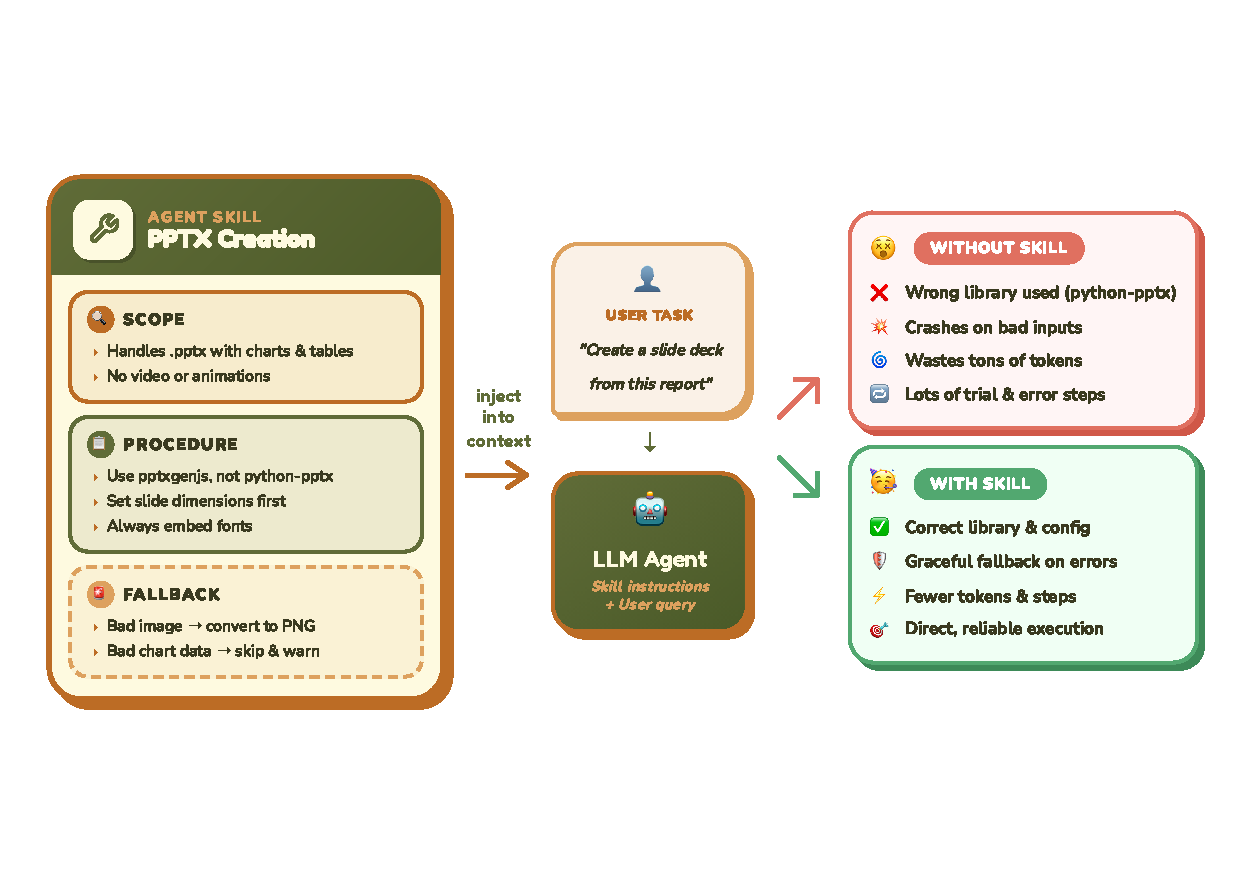
\includegraphics[width=0.99\linewidth]{figs/Agent_Skills.pdf}
    \vspace{-0.2in}
    \caption{Agent Skills are a modular approach that injects domain-specific procedural knowledge (scope, instructions, and fallback conditions) into the agent's context at inference time, bridging the gap between knowledge and reliable execution.}
    \vspace{-0.2in}
    \label{fig:concept}
\end{figure}



%% we should have an introduction section, discussing the motivation of this paper, highlighting the contribution of this paper

\section{Introduction}

LLM-based agents have demonstrated broad competence across many tasks \cite{guo2024large}. At the same time, the research community has identified recurring limitations when these agents are deployed on specialized, real-world workflows \cite{lin2025llm,li2024survey}. 
A substantial body of work has sought to close this gap through three main strategies: retrieval-augmented generation (RAG), domain-specific fine-tuning, and tool-integration frameworks such as MCP.
These methods improve access to knowledge, specialized behavior, and external functionality, respectively. However, they do not fully solve a core problem: many real-world failures arise not from missing facts or missing tools, but from missing procedural knowledge about how to use them effectively and reliably.


This observation has recently motivated fast growing interest in \textbf{agent skills}: one major \emph{skills} marketplace grew from 2{,}179 to over 40{,}000 public skills in just 20 days~\cite{ling2026skillsanalysis}, and the \texttt{anthropics/skills} repository accumulated over 62{,}000 GitHub stars within four months of launch~\cite{xuyan2026survey}. In October 2025,  Anthropic introduced \emph{skills} as organized folders of instructions, scripts, and resources that Claude can load dynamically for specialized tasks, and by December 2025 had expanded the idea into organization-wide deployment features and an open Agent \emph{skills} standard~\cite{xuyan2026survey}.
An \emph{agent skill} can be viewed as a modular, filesystem-based package of domain-specific procedural knowledge that an agent loads at inference time to alter how it behaves on a task, as shown in Fig. \ref{fig:concept}. Conceptually, a \emph{skill} is like a cooking recipe for an agent: rather than supplying new ingredients or kitchen tools, it provides procedural guidance for how available knowledge, tools, scripts, and references should be combined to reliably produce a desired outcome.
Early evidence suggests that this skill-based abstraction is promising: SkillsBench evaluates skills on 86 tasks across 11 domains and finds that curated skills improve average pass rate by 16.2 percentage points \cite{skillsbench2026}. 
OpenAI now describes skills as a way to package task-specific capabilities and share them across teams or with the broader community. 
At the same time, this rapid growth raises important open questions:  
What bottlenecks in current LLM agents can skills address, and where do they fall short? 
How should skills be developed, discovered, evaluated, governed, and secured~\cite{xuyan2026survey, jiang2026sok}?

These rapid developments and open questions motivate us to present this paper.   
We argue that skills should be studied not as a minor implementation detail, but as a distinct systems layer for agentic AI. We first examine the structural bottlenecks that limit current LLM agents,  then discuss how skills may help address some of these limitations and outline  major open questions about skills. Finally, we call for further contributions  to this emerging area.

We believe this blue-sky paper is valuable because it helps define an emerging area before it becomes dominated by fragmented practice. By clarifying the role of skills in LLM agents, identifying their promise and limitations, and laying out a research roadmap, the paper provides a useful foundation for future work on more reliable, reusable, and domain-specialized agent systems.
% ================================================================
% §1  BOTTLENECKS
% ================================================================
\section{Structural Bottlenecks of LLM Agents}
\label{sec:bottlenecks}

Three bottlenecks are widely observed and persist under current scaling paradigms.


\paragraph{\textbf{1) Diminishing Returns from Scaling}}
\label{sec:scaling}Both pre-training and post-training are approaching practical limits. On the pre-training side, each order-of-magnitude increase in compute produces diminishing improvements. Each incremental accuracy gain on challenging benchmarks requires disproportionately more compute than the previous~\cite{scalingwall2025}. Post-training via reinforcement learning has improved reasoning on tasks with verifiable reward signals such as mathematics and code~\cite{guo2025deepseek}. However, these gains do not transfer reliably to open-ended professional workflows \cite{huan2025does,yue2025does}.


Benchmark trajectories on realistic agent tasks show a decelerating pattern. On WebArena, the best agent improved from 14.4\% (2023) to 57.1\% by mid-2024, a gain of 42.7 percentage points in roughly one year~\cite{webarena2023}.\footnote{57.1\% achieved by Jace AI AWA-1.5, August 2024; see WebArena leaderboard.} The bulk of the gains came in a single burst driven by architectural innovation. Progress has continued but at a markedly slower rate: the subsequent eighteen months added approximately 15 percentage points. According to the insights from Anthropic CEO Dario Amodei, while the initial "low-hanging fruit" of language modeling has been harvested through massive web-crawling, the industry is entering a more nuanced phase. The trajectory suggests that the easiest gains from raw data ingestion have been captured, and further improvement increasingly depends on factors beyond simple model scaling~\cite{amodei2023dwarkesh}.


\paragraph{\textbf{2) Context Inefficiency}}
\label{sec:context}Current agents waste a large fraction of their context budget on redundant information, failed attempts, and verbose tool outputs. In a study of software engineering agent sessions, the average task consumed 48,400 tokens across 40 interaction steps, with tool outputs accounting for 63\% of all context~\cite{agentdiet2025}.

This inefficiency compounds as context grows. In mid-2025, across 18 state-of-the-art models, accuracy degrades significantly as context length increases beyond the models' reliable operating range, with performance dropping by 20--50\% on retrieval tasks at longer contexts~\cite{contextrot2025}. The problem is worsening: over the period ending in late 2025, average prompt lengths grew from around 1,500 to over 6,000 tokens (roughly fourfold), reflecting the increasing complexity of agent tasks~\cite{openrouter2026}.
Context is not merely a convenience. It is a hard budget. Every token spent on a failed attempt or irrelevant tool output is a token unavailable for productive reasoning. As agents tackle more complex multi-step tasks, this inefficiency becomes a binding constraint.




\paragraph{\textbf{3) The Reasoning-Execution Gap}}
\label{sec:gap}
Frontier models now exceed 90\% on AIME 2025, a highly selective mathematics competition where even top-1\% human participants score around 84\%~\cite{matharena2025}. Yet high peak performance masks a deeper problem: \textit{reliability}. 
A model may succeed at least once in  k attempts, yielding a high  pass@k, while still failing to solve the task  consistently across repeated  $k$ trials, yielding a low consistency-oriented metric such as pass$^k$ ~\cite{yao2024bench}. Reasoning proficiency, therefore, does not ensure reliable task execution. When models face specialized workflows requiring multi-step procedural planning, both average accuracy and consistency drop sharply.  In medicine, LLMs score 84--90\% on knowledge assessments but only 45--69\% on practice-based tasks requiring multi-step procedural execution~\cite{jmir2025medical}. In chemical synthesis, LLMs achieve only a 47--51\% solve rate without augmented search~\cite{synthelite2025}. On FinanceQA, they fail on approximately 60\% of tasks~\cite{financeqa2025}.


The bottleneck appears epistemological rather than computational: domain-specialized 8B-parameter models collectively outperform general-purpose 110B+ models on corresponding tasks~\cite{learnware2025}. External procedural modules consistently fill this gap, with gains up to 15~pp from code interpreters on mathematical reasoning tasks ~\cite{gao2023pal} and 5.5--13$\times$ error reduction from clinical tools~\cite{clinicalcalc2025}.







%\paragraph{Broader challenges.} Beyond these three bottlenecks, LLM agents face challenges that no single approach can fully address. Agents frequently disregard safety constraints during tool calls, with an average safety score of only 38.5\% across 16 evaluated agents and no agent exceeding 60\%~\cite{agentsafetybench2024}. Hallucination propagates across multi-step agent workflows---even the best models localize only 41.1\% of hallucination sources in agent trajectories---and cannot be eliminated by procedural guidance alone~\cite{agenthallu2026}. Unified evaluation frameworks for real-world agent deployment remain lacking, with current benchmarks fragmented across incomparable, researcher-specific designs~\cite{agenteval2026}. These challenges require complementary research directions in alignment, robustness, and evaluation methodology. The research agenda proposed in this paper targets the procedural knowledge gap specifically and does not claim to resolve these orthogonal issues.



% ================================================================
% §2  SKILLS AS RESPONSE
% ================================================================
\section{Agent Skills as Procedural Knowledge}
\label{sec:skills}

The above bottlenecks suggest that current LLM agents are limited not only by missing knowledge or missing tools, but also by missing procedural knowledge. While RAG, fine-tuning, and MCP-based tool use address part of this gap, they do not fully solve it. This motivates agent skills as a complementary abstraction for encoding and reusing task-specific procedures at inference time.
%Multiple approaches can address the procedural knowledge supply gap identified in \S\ref{sec:bottlenecks}: retrieval-augmented generation (RAG), domain-specific fine-tuning, tool routing via protocols such as MCP. Agent Skills are one promising direction among these alternatives.

\paragraph{Definition.} An Agent \emph{skill} is a modular, filesystem-based package of domain-specific procedural knowledge that an agent loads at inference time to modify its execution behavior~\cite{xuyan2026survey}. A \emph{skill} minimally comprises three observable components: (1)~a \emph{scope declaration} specifying what the \emph{skill} does and does not cover, (2)~\emph{procedural instructions} encoding domain workflows in structured natural language, and (3)~\emph{failure and fallback conditions} specifying when the \emph{skill} should not act and how to retreat. Skills are different from passive retrieval results (RAG), single-function API calls (tools), and weight modifications (fine-tuning), as compared in (Table~\ref{tab:comparison_comprehensive}).  During execution, a \emph{skill} is activated when the current task matches its declared scope. Once loaded, it influences the agent's subsequent decisions, including action selection, tool usage, and stopping behavior. For instance, a pptx \emph{skill}~\footnote{\url{https://github.com/anthropics/skills/blob/main/skills/pptx/pptxgenjs.md}} may restrict itself to slide construction, encode procedures for creating and organizing slides via PptxGenJS, and specify fallback behavior when required dependencies are unavailable.

% For example, a \texttt{pptx} Skill~\footnote{\url{https://github.com/anthropics/skills/blob/main/skills/pptx/pptxgenjs.md}} illustrates all three components: its \emph{scope declaration} limits coverage to PowerPoint generation via PptxGenJS; its \emph{procedural instructions} walk the agent through initializing a presentation, adding slides, and embedding content; and its \emph{failure conditions} specify when to abort, such as when the library is unavailable.



%context for the duration of a session: it persists across steps, encodes when \emph{not} to act, and composes with other Skills. Three necessary conditions distinguish Skills from prompt libraries or instruction templates: (a)~the contractual components (scope declaration, failure conditions) are mandatory, not optional metadata; (b)~composition and conflict resolution are first-class interface concerns, meaning Skills must declare preconditions and side effects to enable principled multi-Skill interaction; and (c)~session-level behavioral impact---the extent to which a loaded Skill reshapes the agent's decision distribution across an entire session---must be observable and measurable, not merely assumed.




%\paragraph{Objective.} The goal is to maximize domain task success rate under two hard constraints: a finite context-token budget and acceptable safety risk. Skills contribute to this objective by supplying procedural knowledge that the model lacks, in a format that is context-efficient and composable. Skills are not designed to solve safety alignment, general reasoning, or hallucination suppression directly---these require dedicated research directions. Whether domain-specific Skills can contribute to these goals (e.g., a safety-checking Skill or a hallucination-detection Skill) remains an open question (Table~\ref{tab:comparison_comprehensive}).





% \newcommand{\yes}{\checkmark}
% \newcommand{\no}{$\times$}
% \newcommand{\maybe}{$\sim$}
\newcommand{\unknown}{\faQuestionCircle} 

\begin{table*}[t]
\centering
\caption{Comparison of skills and other approaches. \yes~= yes; \no~= no; \maybe~= partial/different in kind; \unknown~= unexplored. } %Skills are evaluated alongside existing paradigms like RAG and Tools. }
\label{tab:comparison_comprehensive}
\vspace{-0.1in}
\small 
\resizebox{1.8\columnwidth}{!}{
\begin{tabular*}{\textwidth}{@{\extracolsep{\fill}}l c c c c c c c c c@{}}
\toprule
\textbf{Approach} & 
\makecell{\textbf{Training-free}} & 
\makecell{\textbf{Knowledge}\\\textbf{Enhanced}} & 
\makecell{\textbf{Compos-}\\\textbf{ability}} & 
\makecell{\textbf{Community}\\\textbf{Contrib.}} & 
\makecell{\textbf{Context}\\\textbf{Efficiency}} & 
\makecell{\textbf{Active }\\\textbf{Exploration}} & 
\makecell{\textbf{Planning \&}\\\textbf{Reasoning}} & 
\makecell{\textbf{Safety}} & 
\makecell{\textbf{Hallucination}\\\textbf{Mitigation}} \\
\midrule
RAG             & \yes  & \yes    & \no    & \maybe & \no    & \no    & \no    & \maybe   & \yes  \\
Tools / MCP     & \maybe  & \maybe & \maybe & \yes   & \maybe & \no    & \maybe & \maybe & \maybe \\
Fine-tuning     & \no   & \maybe & \no    & \no    & \maybe   & \no & \maybe & \maybe & \no    \\
\midrule
\textbf{Skills} & \yes  & \yes   & \yes   & \yes   & \yes   & \yes   & \unknown & \unknown & \unknown \\
\bottomrule
\end{tabular*}}
\vspace{-0.1in}
\end{table*}



A key feature of a \emph{skill} is that it reshapes the agent's execution behavior across an entire session, not just at a single step. It can persist across actions, specify when not to act, and compose with other \emph{skills}. This makes \emph{skills} more than prompt libraries or instruction templates.  First, key elements such as scope and failure conditions should be explicit and required. Second, \emph{skills} should support principled composition by declaring preconditions and side effects. Third, their effect on agent behavior should be observable and measurable across the full session.
Together, these properties ensure that \emph{skills} function as reliable, reusable, and analyzable components of agent behavior, rather than as ad hoc prompt fragments.
In this way, \emph{skills} can support agent systems by providing procedural knowledge that the model lacks in a context-efficient and composable form, as detailed next.
Whether \emph{skills} can also help address broader challenges such as safety alignment or hallucination suppression remains an open question.

\vspace{-4pt}
\subsection{Skills Bridge the Knowledge--Practice Gap}
\label{sec:skills-gap}

Skills provide domain-specific procedural knowledge at inference time without retraining, potentially helping agents follow effective workflows and avoid known failure modes. SkillsBench~\cite{skillsbench2026} provides initial empirical evidence across 86 tasks, 11 domains, and 7,308 agent trajectories. Curated \emph{skills} improve absolute pass rates by an average of 16.2 percentage points. Yet the gains varied widely across domain: from +4.5~pp in software engineering to  +51.9~pp in healthcare. %This variation suggests that domain-specific procedural knowledge supply is an important factor, though confounders such as task difficulty and baseline performance across domains have not been controlled. Focused Skills containing 2--3 modules consistently outperform broader alternatives. 
SkillsBench also found that focused \emph{skills} with 2--3 modules outperformed broader alternatives, while auto-generated \emph{skills} showed no average benefit. 
Together, these findings suggest that high-quality, domain-specific procedural knowledge matters.
%, suggesting that current automated methods do not yet produce effective Skills. Whether the bottleneck is generation methodology or the absence of domain-specific procedural knowledge remains open.

%These results are correlational. They show that Skills are associated with performance gains but do not establish a causal mechanism. Whether the gains arise from procedural guidance, reduced search space, or improved prompt structure remains open.

\paragraph{Why skills may bridge this gap.} Both inference-time scaling and \emph{skills} improve task performance without modifying model weights, but through different mechanisms. Inference-time scaling expands the search space through additional computation (e.g., tree search, repeated sampling). Skills instead provide procedural knowledge that narrows this search, steering agents toward effective workflows and away from known failure modes
%Skills take a complementary approach: they encode procedural knowledge distilled from practitioner experience, directing the agent toward proven execution paths and away from known failure modes.
\footnote{See ``Common Pitfalls'' \href{https://github.com/anthropics/skills/blob/main/skills/pptx/pptxgenjs.md\#common-pitfalls}{Anthropic Skills Repository.} }
In this sense, \emph{skills} do not replace compute, but can make it more efficient by improving the quality of the agent's decisions at each step.
Just like the cooking recipe: it encodes procedural knowledge in a reusable form that anyone can follow without understanding the underlying chemistry. Skills work the same way, packaging domain procedural knowledge into portable files any agent can load at inference time. A community-built ecosystem amplifies this advantage, letting practitioners collectively author and share \emph{skills}, turning specialized expertise into reusable infrastructure for many agents.

%Where compute scaling often involves a vast search over potentially meaningless attempts, Skills make each step more likely to succeed. 
%A community-built Skills ecosystem amplifies this advantage: practitioners collectively encode, test, and refine domain procedures, creating a distributed, inference-time knowledge base that other agents reuse.

\vspace{-4pt}
\subsection{Skills Improve Context Efficiency}
\label{sec:skills-context}

Skills address the context inefficiency bottleneck (\S\ref{sec:context}) through progressive loading: only metadata is loaded at startup; full instructions are read on demand; bundled resources are accessed as needed. This effectively decouples capability breadth from context cost.

As empirical support, SAGE~\cite{sage2025} shows that reusing a learned \emph{skill} library reduces interaction steps by 26\% and generated tokens by 59\%. SkillRL~\cite{skillrl2026} further shows that distilling agent trajectories into compact, reusable \emph{skills} can reduce context length by about 10\% while improving task performance by over 15\%. %The mechanism is direct: explicit procedural guidelines eliminate unnecessary exploration and backtracking---the primary drivers of context waste identified in \S\ref{sec:context}. SkillsBench further confirms that focused Skills (2--3 modules) consistently outperform broad alternatives, suggesting that precise procedural guidance is more context-efficient than bulk information loading.
Taken together, these results suggest that \emph{skills} improve context efficiency by replacing unnecessary exploration and backtracking with compact procedural guidance. In this sense, precise \emph{skills} can be more context-efficient than loading large amounts of undifferentiated information.


\vspace{-6pt}
\subsection{Skills Expand Agent Capabilities}
%Extend the Agent's Native Capability Boundary}
\label{sec:skills-extend}

Just as calculators expand an LLM's ability to perform precise arithmetic and code interpreters expand its ability to execute computation, \emph{skills}  can expand what an agent is able to do in specialized domains by supplying reusable domain procedures that it cannot reliably execute on its own.% the ability to execute domain procedures they cannot perform natively.

Prior work offers early evidence for this view.
Voyager~\cite{wang2024voyager} shows that agents equipped with accumulated \emph{skill} libraries achieve 3.3$\times$ more unique items and explore 2.3$\times$ farther in open-ended environments, effectively unlocking task opportunities  that agents without \emph{skills} cannot access. %Each acquired Skill expands the range of subsequent tasks the agent can attempt, creating compound capability growth.
A key reason is that \emph{skills} package reusable procedural knowledge.
Such procedural structure can itself drive performance gains. Hierarchical task decompositions enable 
%Procedural knowledge encoded as hierarchical task decompositions enables 
20--70B parameter models to outperform 120B models lacking such structure~\cite{htn2025}, showing that explicit step orderings, preconditions, and subgoals can matter more than additional scale alone. 
%Procedural decomposition provides explicit task structure---step ordering, preconditions, and sub-goal definitions---that models cannot reliably derive from first principles. The advantage comes from knowledge organization, not parameter count.
A similar pattern appears in clinical settings, where task-specific  calculation tools reduce LLM error rates by 5.5--13$\times$ \cite{clinicalcalc2025}. These tools encode domain procedures such as calculation sequences, unit conversions, clinical decision thresholds that general-purpose reasoning alone cannot reliably execute. 
%This is the reasoning-execution gap from \S\ref{sec:gap} in microcosm: the model possesses relevant knowledge but lacks the procedural scaffolding to apply it reliably.
These results highlight how \emph{skills} can expand agent capabilities by helping bridge the reasoning--execution gap identified in \S2.



% ================================================================
% §3  OPEN QUESTIONS
% ================================================================


\vspace{-6pt}
\section{Open Questions}
\label{sec:qs}
As a new and rapidly growing area, agent \emph{skills} are attracting increasing attention across both research and practice, yet many of their core questions remain unresolved. We identify  10 questions   spanning three broad areas: runtime \emph{skill} use, \emph{skill} construction, and \emph{skill} quality estimation and trust.
 
%Despite the rapid evolution of decentralized ecosystems, the community-contributed Agent Skills layer remains a nascent field. \hm{We identify 8 open questions for agent skills development.}
% We propose six research directions to bridge this gap, addressing systemic challenges that have yet to be rigorously examined by the academic community.

% \paragraph{Three hard constraints.} One might ask whether Skills ecosystem challenges reduce to familiar problems in software engineering (package management) or information retrieval (semantic search). Three constraints unique to the Skills setting explain why existing solutions are insufficient:

% \begin{enumerate}
%   \item[\textbf{C1.}] \textbf{Context budget as hard cost.} A retrieval error consumes tokens irreversibly, destroying downstream reasoning capacity. Concretely, an irrelevant Skill injected into context displaces tokens that could have carried productive instructions, and no mechanism exists to reclaim that capacity mid-session.
%   \item[\textbf{C2.}] \textbf{Session-level behavioral impact.} In-context instructions condition all subsequent model outputs~\cite{brown2020language}. A loaded Skill therefore reshapes the agent's decision distribution for the remainder of the session. Unlike a one-shot tool call, a selection error compounds through every subsequent decision rather than being isolated.

%   \item[\textbf{C3.}] \textbf{Natural-language contracts resist full formalization.} Critical Skill behaviors (when \emph{not} to act, how to handle ambiguity, when to retreat) are expressed in natural language and cannot be fully reduced to code.
% \end{enumerate}

% These constraints interact: C1 makes retrieval errors costly, C2 makes them persistent, and C3 makes them hard to prevent through formal verification. Each Research Question (RQ) below states the problem, explains why it is difficult, identifies what exists and what is missing, and highlights what is new in the Skills setting.

% We identify six research questions that, linked by the three hard constraints unique to the Skills setting (C1–C3), unfold in a natural dependency order. The chain begins at the foundation: before any ecosystem can function, the community must agree on what a Skill is and how Skills interact—this is the domain of RQ1 (Granularity and Composition)—and must be able to measure whether a Skill actually works, which is the domain of RQ2 (Evaluation). These two questions are prerequisite to all others; without contract interfaces and evaluation protocols, the remaining questions lack the vocabulary and metrics needed to make progress. Once contracts and evaluation exist, three ecosystem-level challenges become tractable in parallel: RQ3 (Safety Trust) asks whether a Skill's behavioral impact can be verified as benign; RQ4 (Discovery and Selection) asks how an agent should choose among Skills under a finite context budget; and RQ5 (Behavioral Portability) asks whether a Skill that works on one model transfers reliably to another. All three depend on the contract metadata and quality signals established by RQ3 and RQ5. Finally, RQ6 (Governance) sits as the capstone: even a technically sound ecosystem collapses if it cannot sustain contributor incentives or resist vendor consolidation, making governance the question that determines whether the entire structure endures as a public good.

% \paragraph{Window of opportunity.} The skills ecosystem is currently in its early stages, with no dominant standards yet in place. This is the critical window where research acts as a ``GPS'' for the ecosystem. Without the guidance of rigorous research, development often becomes a blind race, leading to costly mistakes and "dead-end" technology paths. By investing in research now—while protocols and governance are still being shaped—we can ensure the development stays on the right track. It is far cheaper to guide the design today than to fix a broken, locked-in system tomorrow.

\vspace{-8pt}
\subsection{ Runtime Skills Use}

\hspace{\parindent}\emph{\textbf{Q1: How to select  skills }} % Skill Discovery and Selection.} How to select and sequence Skills from a large-scale registry?}\label{sec:q1}

% No dedicated registry exists (\textcolor{red}{For your reference: \url{https://github.com/LabRAI/LangSkills}}).
Skills are rapidly accumulating across GitHub repositories and dedicated platforms~\cite{langskills,skillsmp,skillsrest,clawhub}, contributed by developers, organizations, and broader user communities. In practice, however, skill selection still relies heavily on popularity signals, e.g., GitHub star counts and ClawHub stars. Although such metrics are convenient and visible, they are imperfect proxies for actual utility: prior work shows that stars correlate only moderately with development activity ($\rho = 0.44$ with commits) and exhibit little  relationship with intrinsic code quality~\cite{borges2018stars, sajnani2014popularity}. Moreover, star-based metrics are susceptible to manipulation %; recent measurements report millions of suspected fake stars on GitHub
~\cite{he2026fakestars}. This limitation is further amplified by the cold-start problem, since newly published skills may have little or no ecosystem activity from which popularity can be inferred.

Although recent work has begun to study ecosystem-scale orchestration across 200K Skills~\cite{agentskillos2026}, the main discovery problem remains open. Unlike RAG~\cite{lewis2020rag} or tool-augmented systems~\cite{schick2023toolformer}, where retrieved items are often independent, agents may load multiple skills into a shared session context. Co-loaded skills may complement, overlap, or conflict, and a poor early choice can propagate errors through the session~\cite{furuta2024compwob}.
This calls for discovery methods that jointly optimize task benefit, context cost, and multi-skill interaction, rather than relying on standard popularity-based ranking.


% The de facto quality signal, GitHub star count, correlates only weakly with development activity ($\rho = 0.44$ with commits) and not at all with code quality~\cite{borges2018stars, sajnani2014popularity}. Star counts are also manipulable: approximately 3.8 million confirmed fake stars have been identified on GitHub~\cite{he2026fakestars}. Cold start compounds the problem. Quality signals depend on ecosystem activity that does not yet exist. \textcolor{red}{(This paragraph is informal.)}



%Existing information retrieval and recommender-system techniques are optimized for retrieval and ranking at scale. However, the \emph{Skills} setting introduces a fundamental difference: unlike RAG~\cite{lewis2020rag} or tool-augmented systems~\cite{schick2023toolformer} that retrieve independent, stateless results, agents typically load multiple \emph{Skills} simultaneously into a shared session context. This transforms the problem from single-item retrieval into \emph{portfolio selection with interaction effects}. Co-loaded \emph{Skills} influence each other---their instructions may reinforce, overlap, or contradict---and a poor selection at an early stage can propagate errors through subsequent decisions, causing compositional task performance to degrade sharply relative to single-task baselines~\cite{furuta2024compwob}. Each retrieval error carries quantifiable opportunity cost and persists through the session. This demands a new discovery objective that jointly optimizes task performance gain, context token cost, and multi-skill interaction conflict---criteria that standard IR ranking does not capture.



\vspace{+0.04in}
\emph{\textbf{Q2: Reliability vs. Variety, can skills achieve both?}}\label{sec:q2}

Procedural instructions in \emph{skills} can improve the reliability of agent outputs, but they may also reduce output diversity. This is particularly visible in pptx \emph{skills}, where detailed step-by-step guidance can narrow the range of acceptable designs and cause presentations to converge on similar layouts, structures, and rhetorical styles. In this way, stronger procedural control may come at the cost of creative variation. This concern echoes the “Artificial Hivemind” effect, in which language models tend to produce increasingly similar open-ended outputs~\cite{jiang2025artificial}. A central open question, therefore, is how much procedural structure is needed to improve reliability without overly constraining diversity.



\vspace{+0.04in}
\emph{\textbf{Q3: How to prevent skill overreach? }}\label{sec:q3}

Since a loaded \emph{skill} persists across an entire session, its influence may extend beyond its declared scope. For example, a medical diagnosis \emph{skill}  may make an agent more conservative or disclaimer-prone even when it later performs an unrelated task such as code generation. This is not a conflict between multiple \emph{skills} or a failure within the \emph{skill}'s intended scope, but a form of \textbf{behavioral spillover}: because in-context instructions and prompt format alone can shift behavior substantially~\cite{brown2020language,sclar2024prompt}, a loaded \emph{skill} may act beyond its intended boundaries. How to detect, quantify, and suppress such spillover is an open question.
Declaring scope boundaries is insufficient, because a \emph{skill}'s boundaries are themselves instructions interpreted by the model, not hard execution constraints.

\vspace{+0.04in}
\emph{\textbf{Q4: Where do skills help most? }}  

Skills provide task-specific procedural scaffolding, but they are not a substitute for general reasoning, planning, or safety mechanisms (Table~\ref{tab:comparison_comprehensive}). A \emph{skill} can shape action selection and workflow structure, but it does not by itself ensure correct reasoning, factual accuracy, or safe behavior. Moreover, the benefits of \emph{skills} appear highly domain-dependent: while curated \emph{skills} improve average performance, the size of these gains varies widely across domains~\cite{skillsbench2026}.
Therefore, an important open question is where \emph{skills}  can help, and where they cannot.

\vspace{-7pt}
\subsection{Skills Construction}

\hspace{\parindent}\emph{\textbf{Q5: How should skill scope and composition be defined? }}
%Granularity and Composition Interfaces.} How should the minimal reusable \emph{Skill} unit be defined, and how should multi-\emph{Skill} composition conflicts be resolved?}
\label{sec:q5}

A key open question is how granular a skill should be. Too fine-grained, and \emph{skills} become trivial wrappers with brittle dependencies~\cite{abdalkareem2017trivial}; too coarse, and they become monolithic and hard to compose or reuse. In the recipe analogy, the issue is not only whether strawberry cake and blueberry cake should be treated as separate recipes, but also where exactly one recipe should end: at baking, or also at frosting, decoration, and final serving?

When multiple \emph{skills}  interact, the challenge becomes deeper. Unlike software components, \emph{skills} lack formal type systems: their scope, preconditions, and side effects are expressed in natural language, making conflicts semantic, context-dependent, and difficult to detect automatically. As a result, software granularity conventions~\cite{decan2019emse} may not transfer directly. Skill composition is therefore not just an interface-design problem, but an open NLP problem: how can usable skill boundaries and composition rules be defined   when the ``type system'' is natural language.

%Two failure modes bracket the problem of defining \emph{Skill} scope. At one extreme are overly fine-grained \emph{Skills}, analogous to npm-style trivial packages, where 16.8\% of packages are single-function wrappers~\cite{abdalkareem2017trivial}, creating fragile dependency chains. At the other extreme are overly coarse \emph{Skills} that become monolithic, uncompositional, and difficult to maintain. Defining \emph{Skill} scope is like defining a cake recipe: the challenge is not only whether strawberry cake and blueberry cake should be separate recipes, but also whether a recipe should stop at baking the cake itself or extend to frosting, decoration, serving, and presentation. 
% Two failure modes bracket the problem. Too fine-grained: npm-style trivial packages, where 16.8\% of packages are single-function wrappers~\cite{abdalkareem2017trivial}, creating fragile dependency chains. Too coarse: monolithic Skills that are uncompositional and unmaintainable. The right granularity depends on domain-specific task decomposition.

%The deeper challenge is composition conflict. In software, type systems detect interface mismatches at compile time. Skills lack any equivalent: their preconditions, side effects, and scope boundaries are expressed in natural language, where contradictions are semantic, context-dependent, and detectable only through language understanding. This is not an interface engineering problem but an open NLP research question---determining whether two natural-language contracts conflict requires reasoning about entailment, domain-specific logic, and pragmatic implicature simultaneously. Recent proposals for typed abstractions in agent task composition~\cite{jiang2026web} offer a starting point, but \emph{Skills} operate at a higher level of abstraction where full formalization may be impossible~\cite{jiang2026sok}. Existing software granularity conventions~\cite{decan2019emse} inform structural choices, yet the fundamental research question remains: how should composition interfaces work when the ``type system'' is natural language?



\vspace{+0.04in}
\emph{\textbf{Q6: How to ensure skill portability across  models and environments? }} %How can we ensure that the same Skill can be used across different models and agent frameworks?}\label{sec:q5}

\emph{Skills} are structured prompts, so their behavior depends not only on the written specification but also on the underlying model and execution environment. Like the same recipe used in different kitchens, identical instructions may produce different outcomes because the ``ovens,'' ``ingredients,'' and broader operating conditions vary. This makes \emph{skills} inherently vulnerable to both model drift and prompt sensitivity. Prior work shows that GPT-4 accuracy on a simple task dropped from 84\% to 51\% within three months of the same model service~\cite{chen2024chatgptdrift}, and semantically equivalent prompt formats can differ by up to 76 percentage points in accuracy~\cite{sclar2024prompt}.
Existing work studies model drift and prompt sensitivity in isolation, but portability is harder because these factors interact: models may interpret the same instruction differently, required tools may be unavailable, and the target model's knowledge may overlap with or fall short of what the \emph{skill} assumes. Avoid-lists and tool dependencies require model-specific adaptation: an instruction to ``avoid tool X'' is meaningless if the model does not know X exists. Thus, portability is not literal output matching, but \emph{contract satisfaction}: correct behavior, predictable failure modes, and reliable fallback.
 

%This challenge is similar to following the same recipe in different kitchens: ovens heat differently, salt varies in salinity, and ingredients behave differently in practice, even when the written instructions are identical. Likewise, \emph{Skills} are structured prompts, and their behavior depends not only on the written specification but also on the underlying model and execution environment. They inherit both model drift and prompt sensitivity simultaneously. GPT-4's accuracy on a simple task dropped from 84\% to 51\% within three months of the same model service~\cite{chen2024chatgptdrift}. Accuracy varies by up to 76 percentage points between semantically equivalent prompt formats~\cite{sclar2024prompt}. Roughly one-third of software package releases introduce breaking changes, with 14.5\% doing so in minor or patch versions in violation of semantic versioning conventions~\cite{raemaekers2017semver}. Early evaluations confirm these portability challenges: agent skill frameworks show substantially different effectiveness across 12B--80B parameter models in industrial settings~\cite{xu2026slmskills}.


%Existing work studies model drift and prompt sensitivity in isolation. Portability in the \emph{Skills} setting is harder because it decomposes along three dimensions that interact: (1)~\emph{prompt interpretation}---the same natural-language instruction may be understood differently across models; (2)~\emph{capability prerequisites}---a \emph{Skill} requiring a specific tool fails silently if the target model lacks access to it, demanding tool substitution or graceful degradation; and (3)~\emph{knowledge state overlap}---the target model may already embody what the \emph{Skill} teaches (wasting context) or may lack prerequisite knowledge the \emph{Skill} assumes (causing silent failure). Avoid-lists and tool dependencies require model-specific adaptation: an instruction to ``avoid tool X'' is meaningless if the model does not know X exists. The required equivalence is therefore not literal output matching but \emph{contract satisfaction}---correct outputs, consistent failure modes, and equivalent fallback behavior ---diagnosed and tested along each dimension independently.

\vspace{+0.04in}
\emph{\textbf{Q7: How to govern skill ecosystems? }} %Sustainability of Skill Maintenance.} What incentives and governance mechanisms can sustain scarce tacit procedural knowledge as a public good?}\label{sec:q6}


Skills encode non-rival knowledge, but they are costly to create and maintain over time. Their governance challenge is deeper than in traditional open source because the primary bottleneck is often domain expertise rather than coding effort. A clinical diagnostic \emph{skill}, for example, cannot be sustained without medical knowledge. As a result, the most valuable \emph{skills} may also be the most fragile: they depend on rare tacit expertise that is hard to replace once abandoned. Without strong and inclusive governance, \emph{skill} ecosystems may concentrate around a few well-resourced vendors, ultimately recreating the very lock-in that skills were supposed to avoid.

While open-source governance offers useful lessons~\cite{ostrom1990commons,eghbal2016roads}, skills raise additional concerns because their encoded knowledge may be uniquely scarce and irreplaceable. Sixty percent of open-source maintainers are unpaid hobbyists~\cite{tidelift2024maintainer}. Among inactive PyPI developers, 75.4\% never issue deprecation notices~\cite{zhong2025deprecation}.  This makes abandonment, privacy, and liability important for \emph{skills}. A central open question is how to govern \emph{skills} in ways that sustain expertise while preserving openness, accountability, and long-term access.

%Skills encode knowledge that is non-rival (using a \emph{Skill} does not deplete it) but costly to produce and maintain. The governance challenge is deeper than in traditional open source because the \emph{supply-chain bottleneck} differs. A software package can be maintained by any competent developer; a clinical diagnostic \emph{Skill} cannot be maintained without medical expertise. The knowledge supply chain---domain expert $\to$ \emph{Skill}author $\to$ agent $\to$ end user---has its bottleneck at domain expertise, the scarcest and least substitutable resource. This creates an inverse relationship between value and sustainability: the most valuable \emph{Skills} (encoding rare tacit knowledge) are precisely those most vulnerable to abandonment. Without governance, registries and standards will gravitate toward the best-resourced vendor, reproducing the lock-in that \emph{Skills} were meant to avoid.


%Open-source governance research (Ostrom~\cite{ostrom1990commons}, Eghbal~\cite{eghbal2016roads}, Apache model) is extensive. What is new in the \emph{Skills} setting: the knowledge encoded is uniquely scarce and irreplaceable. When a code package is abandoned, substitutes typically exist. When a senior clinician's diagnostic \emph{Skill} is abandoned, the replacement cost is far higher because the tacit knowledge may not exist elsewhere in codified form. Sixty percent of open-source maintainers are unpaid hobbyists~\cite{tidelift2024maintainer}. Among inactive PyPI developers, 75.4\% never issue deprecation notices~\cite{zhong2025deprecation}. New metrics are needed for ``abandonment externality'' and ``knowledge criticality.'' Governance mechanisms must also address data privacy and liability attribution when a \emph{Skill} causes harm.

\vspace{-7pt}
\subsection{Skill Quality Evaluation and Trust}


\hspace{\parindent}\emph{\textbf{Q8: How to evaluate skills across domains?}}
%How can distributed, domain-specific evaluation scale without succumbing to Goodhart's law?}
%\label{sec:q7}

Evaluating a skill is difficult for the same reason that evaluating online recipes is difficult: many alternatives exist, but the right criteria depend on the task, the user’s goals, and the context. Skills make this harder because performance varies widely across domains~\cite{skillsbench2026}, so aggregate metrics are not enough. Meaningful evaluation requires domain-specific task suites, failure taxonomies, and success criteria, yet these depend on the tacit expertise that makes skills valuable. Existing dynamic and community-driven benchmarks~\cite{kiela2021dynabench,srivastava2023beyond,jimenez2024swebench} offer precedent, but skills add two challenges: evaluation is tied to domain authorship, and benchmarks may be gamed as skills improve. The open question is how to build evaluation frameworks that are domain-grounded, robust to gaming, and sustainable.
%A persistent challenge, even for something as seemingly simple as online steak recipes, is who should judge among thousands of alternatives and according to what criteria. Skills face the same problem at larger scale: the 12-fold performance spread across domains in SkillsBench~\cite{skillsbench2026} renders aggregate metrics meaningless. Each domain needs its own task suite, failure taxonomy, and expert-defined success criteria. Constructing these benchmarks requires the same tacit knowledge that makes \emph{Skills} valuable. Evaluation is itself a \emph{Skill}.

%Existing dynamic benchmarks (Dynabench~\cite{kiela2021dynabench}), community-contributed evaluations (BIG-Bench~\cite{srivastava2023beyond}), and real-world task extraction (SWE-bench~\cite{jimenez2024swebench}) provide methodological precedent. Two aspects are new in the \emph{Skills} setting. First, domain success criteria depend on tacit knowledge, making evaluation co-dependent with \emph{Skill} authorship. Second, preventing metric-driven gaming (Goodhart's law) requires co-evolutionary benchmarks that update as \emph{Skills} improve, combined with adversarial probing and expert spot-checks.

\vspace{+0.02in}
\emph{\textbf{Q9: How to secure skills? }} %Safety Trust.} How can malicious manipulation via natural-language instructions and scripts be verifiably detected?}\label{sec:q8}
% \textcolor{red}{I think we should have more discussion on this point. Introducing agent skill to an agentic system or workflows will make larger threat vectors (e.g., prompt injection, jailbreak attack)}

% Skills introduce a sophisticated safety paradigm shift where the threat emerges from the interplay between natural language manipulation and code executability~\cite{jia2026skillject,liu2026malicious,liu2026agent}. This hybridization creates a unique procedural execution trajectory that mirrors the "Foot-in-the-door" multi-turn jailbreak~\cite{weng2025foot}. Rather than a singular, detectable malicious payload, the risk lies in how natural language instructions implicitly reshape the agent’s behavioral distribution over time. By persisting across sessions, a compromised Skill can execute an incremental steering attack—subtly drifting goals and tool-selection patterns across multiple turns. \textcolor{red}{This sentence is not informative. Can you give any examples of that? What's the difference between the threats of skill and threats of other properties within the agentic system?} This cumulative trajectory renders traditional single-turn detection obsolete, as the adversarial intent is atomized into seemingly benign, step-by-step deviations.

Much like food safety in a kitchen, where raw chicken and salad become dangerous once they share the same cutting board, \emph{skills} create new threat pathways by combining familiar attack vectors. They inherit risks such as prompt injection~\cite{debenedetti2024agentdojo}, jailbreaks~\cite{huang2024trustllm,huang2025trustworthiness}, and malicious code execution~\cite{jia2026skillject,liu2026malicious,liu2026agent,mo2025attractive,skillinject2026}, but make them more dangerous by linking natural-language instructions with executable behavior. A malicious \emph{skill} can therefore unfold as a multi-step attack: it may first request plausible permissions, then exploit them to access files, extract sensitive data, or bias future tool use. Because skills are often distributed by third parties yet run with substantial privileges, compromised skills can persist across sessions and steer agent behavior over long horizons. Empirical evidence by early 2026 already showed substantial risk, including high indirect prompt-injection success rates~\cite{zhan2024injecagent}, rapid growth in malicious open-source packages~\cite{sonatype2024ssc}, and tool-poisoning attacks on real MCP servers exceeding 70\% success for some models~\cite{invariant2025toolpoisoning,wang2025mcptox}. This suggests that \emph{skills} introduce not just isolated vulnerabilities, but a new compositional security challenge for agentic systems.

%Much like food safety in a kitchen, where raw chicken and salad are both ordinary ingredients but create a new contamination pathway once they share the same cutting board, \emph{Skills} expand the threat surface by combining otherwise familiar attack vectors. Skills introduce a significant expansion of the threat surface in agentic systems because they inherit and combine multiple previously studied attack vectors, including prompt injection~\cite{debenedetti2024agentdojo}, jailbreak attacks~\cite{huang2024trustllm,huang2025trustworthiness}, and malicious code execution~\cite{jia2026skillject,liu2026malicious,liu2026agent,mo2025attractive,skillinject2026}. Unlike traditional attacks that target a single interaction channel, \emph{Skills} bridge natural language instructions and executable code, allowing adversaries to coordinate attacks across both layers. For example, a malicious \emph{Skill} may initially claim that additional file permissions are required to complete a benign task (e.g., accessing key documents), gradually escalating its access privileges. Once elevated permissions are granted, the \emph{Skill} may then request to read local files under the pretext of retrieving relevant information, while covertly extracting sensitive data such as stored API keys (e.g., GPT API credentials) or private documents. This hybridization creates a procedural execution trajectory that mirrors the "Foot-in-the-door" multi-turn jailbreak~\cite{weng2025foot}, where each step appears benign but collectively leads to policy violations. The key difference between \emph{Skills} and other components in agentic systems is their distribution and privilege model. Skills are often developed and published by third-party contributors with limited oversight, yet they execute directly on user devices or backend servers where agents are frequently granted high-level permissions. As a result, compromised \emph{Skills} can persist across sessions and gradually manipulate task objectives or tool-selection behaviors, enabling long-horizon steering attacks that are difficult to detect through traditional single-turn safety mechanisms.



%The evidence of the threat was concrete by early 2026. LLM agents are vulnerable to indirect prompt injection at rates of 24\% (GPT-4 baseline), rising to 47\% (GPT-4) and up to 88.2\% (Llama2-70B) under adversarial settings~\cite{zhan2024injecagent}. Malicious packages in open-source registries have reached 704,000 cumulative, growing 156\% year-over-year~\cite{sonatype2024ssc}. Tool poisoning attacks on real MCP servers exceed 70\% success rate for some models~\cite{invariant2025toolpoisoning, wang2025mcptox}.

\vspace{+0.02in}
\emph{\textbf{Q10: 
Will skill-based training cause procedural collapse?}}
%Skills as Training Data.} Can Skills serve as high-quality training corpora, and how can they be used to evolve the next generation of models?}\label{sec:qx}

As the number of \emph{skills} grows to 400,000~\cite{skillsmp} and growing, they are becoming a large-scale training resource. This raises an open question: can \emph{skills} serve as training data for future models, and if so, what can models learn from them? Because \emph{skills} encode canonical procedures, expert-preferred decompositions, and normative task formats, they may overweight already-salient problems while compressing long-tail variation. The risk is greater if models are trained on \emph{skills} without trajectories or other records of situated execution: they may learn procedural templates, but not the fuller behavioral distribution needed for adaptation and recovery. This suggests a possible recursive-training failure mode in which models collapse not only through synthetic data, but toward a narrower and more homogeneous procedural canon~\cite{wu2024generative,shumailov2024ai,jiang2025artificial}. The challenge is how to leverage \emph{skills} to improve models without amplifying monoculture, long-tail loss, or overconvergence.




% \subsection{Q10: Process Compliance Monitoring}
% \label{sec:q10}

% \emph{Can an agent reliably detect whether it is faithfully following a Skill's procedural steps, rather than merely producing plausible outputs through its own capabilities?}

% Q2 asks whether a Skill improves outcomes. Q10 asks a different question: whether the Skill's procedure was actually followed. These are not the same. An agent may produce a correct result through its own parametric knowledge while ignoring the Skill entirely. Conversely, an agent may believe it is following the Skill while silently deviating at intermediate steps. Without process-level monitoring, it is impossible to distinguish Skill-caused improvement from coincidental improvement~\cite{skillsbench2026}. This matters because the entire empirical case for Skills rests on the assumption that loaded Skills shape agent behavior. If agents do not reliably follow procedural instructions, the evaluation results in Q2 lose their interpretability.

% The challenge is deeper than it appears. Skills encode multi-step procedures, and compliance must be assessed step by step, not just at the final output. Recent work on process reward models shows that outcome supervision alone is insufficient to verify correct reasoning chains~\cite{lightman2023verify}. The Skills setting is harder still: procedural compliance is expressed in natural language, so deviations are semantic rather than syntactic and cannot be detected through simple string matching. A dedicated framework for Skill-level process supervision is an open problem.

\vspace{-8pt}
\section{A Call for Contribution}
The rapid growth of the skills ecosystem—from a handful of curated packages to over 400,000 public Skills in months—signals genuine demand, yet the infrastructure to make it reliable, safe, and sustainable does not yet exist. If the community addresses the open questions in Section 4, the impact will unfold across two horizons.
In the near term, \emph{skills} let agents reach expert-level execution that raw scaling cannot: a clinical agent that follows verified diagnostic workflows rather than hallucinating procedures, a synthesis agent that executes feasible chemical routes rather than plausible-sounding ones, a financial agent that applies precise domain logic rather than approximate reasoning—gains that come not from a larger model but from procedural expertise loaded on demand.

In the longer term, the paradigm opens an ambitious possibility: agents that not only consume \emph{skills} but create, evaluate, and evolve them~\cite{skillrl2026,yang2026autoskill}—distilling completed tasks into reusable \emph{skills}, revising procedures after failures, and collectively improving a shared library. This self-evolving loop, where agents become both users and authors of procedural knowledge, marks a shift from static tool use toward a living, self-improving knowledge infrastructure.

Realizing either horizon requires foundational research that the community has not yet undertaken. We therefore outline a call for contribution from three complementary perspectives.

\vspace{-0.05in}
\paragraph{\textbf{The Skill developer's perspective}} The ask is simple: follow emerging standards and share \emph{skills} openly. A well-scoped, clearly documented \emph{skill} in a public registry does not just help one agent; it becomes reusable infrastructure for many. The more developers treat \emph{skills} as a \textbf{shared knowledge commons} rather than proprietary artifacts, the faster the ecosystem accumulates value.

\vspace{-0.05in}
\paragraph{\textbf{The Skill user's perspective}} 
The ask is to treat \emph{skills} as a first-class mechanism for extending agent capability, learn to select and compose them effectively, and report failures. When a user reports that a \emph{skill} misbehaves, interferes with adjacent tasks, or breaks under certain conditions, that feedback improves not just one interaction but the reliability of the broader ecosystem.

 
\vspace{-0.05in}
\paragraph{\textbf{The researcher's perspective}} The ask is to build the technical and trust foundations that neither developers nor users can build alone: contract schemas that make composition conflicts detectable, discovery systems that rank \emph{skill}  by actual quality rather than star counts, verification pipelines that catch malicious \emph{skill}  before they reach users, and governance models that keep tacit expert knowledge alive and maintained. Without such foundations, the ecosystem will grow fast but remain fragile.
% 

% \vspace{+0.1in}
Whether \emph{skills} become a lasting systems layer or only a transitional pattern remains open. What is already clear is that they force the community to confront a deeper issue: how \textbf{procedural knowledge should be represented, shared, evaluated, and governed in agentic AI}. We hope this paper serves as an invitation to study that question seriously, and in doing so to make agents not only more capable but more understandable, reusable, and trustworthy in the specialized workflows where they are most needed.

%================================================================
% §4  RESEARCH ROADMAP
% ================================================================
% \section{Research Roadmap}
% \hm{I paste the guideline here. Do we still need research roadmap here?}
% \begin{itemize}
%     \item \textcolor{red}{How is the Blue Sky Idea related to the thematic topics of interest for KDD’26? }
%     \item \textcolor{red}{What is the Big and Bold Idea?}
%     \item \textcolor{red}{Why is it a Blue Sky Idea? Why should the community consider it, and why now? Why is it not simply a regular paper submission? }
% \item \textcolor{red}{How does the paper push the frontier, challenge current assumptions, or offer a bold approach to a complex challenge?}
% \item \textcolor{red}{If this idea is successful, what would success look like?}
% \end{itemize}
% \label{sec:roadmap}
% \begin{figure*}
%     \centering
%     \includegraphics[width=1\linewidth]{figs/research_roadmap-3.html.pdf}
%     \caption{Research Roadmap for Agent Skills Development.}
%     \vspace{-0.16in}
%     \label{fig:roadmap}
% \end{figure*}
% The six RQs unfold across three phases as the ecosystem matures. Each phase produces specific outputs that unlock the next.

% \subsection{Phase I: Contracts and Evaluation Foundations}
% \label{sec:phase1}

% \emph{Can start immediately. No ecosystem scale required.}

% This phase addresses RQ1 (granularity and composition) and RQ2 (evaluation). Core tasks include: formalizing \emph{Skill} contract interfaces (scope declarations, preconditions, side effects, rollback semantics), designing a four-dimensional evaluation framework (correctness, efficiency, robustness, composability), establishing baselines using SkillsBench, and deriving initial granularity norms from existing ecosystem data (npm/PyPI module-size distributions).

% \textbf{Dependency arrows.}Without contract interfaces and evaluation protocols, Phase~II cannot define trust scores (RQ3), discovery rankings (RQ4), behavioral equivalence between models (RQ5), or measurable governance targets (RQ6).

% \subsection{Phase II: Community Ecosystem Infrastructure}

% \emph{Unlocked after registries and an initial contributor base form.}

% This phase addresses RQ3 (trust), RQ4 (discovery), RQ5 (portability), and RQ6 (governance). Core tasks include four areas. (1)~Design layered trust verification pipelines building on Phase~I evaluation protocols (static analysis $\to$ sandboxed execution $\to$ peer review $\to$ domain certification). (2)~Build semantic discovery infrastructure using Phase~I contract metadata, including embedding-based retrieval and Skill Cards modeled on Model Cards~\cite{mitchell2019modelcards}. (3)~Develop cross-platform portability standards (precedents: OCI~\cite{oci2015}, LSP~\cite{bunder2019lsp}, ONNX~\cite{bai2019onnx}). (4)~Establish multi-stakeholder governance structures (precedents: Apache Foundation, OpenJS, Python Software Foundation).

% \textbf{Dependency arrows.} Trust requires evaluation protocols (Phase~I). Discovery requires contract metadata (Phase~I). Governance requires measurable indicators (Phase~I).

% \subsection{Phase III: Autonomous Knowledge Evolution}

% \emph{The most speculative and Blue Sky component.}

% The long-term trajectory: from ``humans write everything'' to ``humans write contracts, agents write implementations.'' Practitioners define what to do and what not to do (the contract). Agents generate implementations, generate test cases, verify against the contract, and submit passing implementations for human audit.

% Precedents suggest feasibility. Voyager~\cite{wang2024voyager} demonstrates that LLM agents can autonomously build growing \emph{Skill} libraries in open-ended environments. LATM~\cite{cai2024latm} shows that separating tool-making from tool-using improves performance at lower cost. More recently, AutoSkill~\cite{autoskill2026} demonstrates that agents can autonomously learn and reuse procedural skills from interaction traces without parameter updates, providing early validation for the contract-first development model envisioned in Phase~III. The critical scientific question: how do auto-generated \emph{Skills} avoid mode collapse and gaming of evaluation metrics? How are externalities and liability managed when machine-generated procedural knowledge causes harm?

% The end state is an infrastructure layer for procedural knowledge, analogous to npm/PyPI for software, on which all agents build.

% \paragraph{Falsifiable predictions.}
% \label{sec:predictions}
% \begin{itemize}
%   \item[\textbf{P1.}] Future progress on specialized agent tasks will be better predicted by \emph{Skill} ecosystem metrics (domain coverage, reuse rate, failure rate) than by model benchmark scores alone.
%   \item[\textbf{P2.}] A \emph{Skill} ecosystem lacking supply-side governance will experience vendor lock-in or poisoning attacks faster than traditional software package ecosystems, because session-level behavioral impact amplifies the damage from a single compromised component.
% \end{itemize}
% These predictions are not immediately verifiable but specify observable failure conditions. If within two years neither ecosystem metrics nor poisoning rates differ meaningfully from software package baselines, the urgency of this agenda should be reassessed.


% % ================================================================
% % §5  CONCLUSION
% % ================================================================
% \section{Conclusion}
% \label{sec:conclusion}

% Scaling, whether through larger models, more data, or extended post-training, faces diminishing returns on the procedural knowledge that specialized agent tasks demand. Agent \emph{Skills} offer a promising response: modular, inference-time injection of domain expertise authored by the practitioners who hold it. Early evidence supports the approach, but the ecosystem forming around it faces six open research challenges spanning systems, HCI, security, information retrieval, and governance. These are not downstream engineering problems. They are first-class research questions. Three hard constraints unique to the \emph{Skills} setting distinguish them from prior work: context budget as irreversible cost, session-level behavioral impact, and the inherent informality of natural-language contracts.

% The six RQs are interdependent. Evaluation (RQ2) and contract formalization (RQ1) are foundational; trust (RQ3), discovery (RQ4), portability (RQ5), and governance (RQ6) build upon them. The three-phase roadmap makes these dependencies explicit and identifies what can begin immediately.

% Our agenda rests on three premises: (A1)~an open \emph{Skills} ecosystem will form and sustain itself, (A2)~enough domain practitioners will contribute, and (A3)~models will maintain adequate instruction-following capability. If A1 fails, governance and discovery questions become moot, but evaluation and portability persist. If A3 fails, \emph{Skills} as an architecture may be premature. Two falsifiable predictions (P1, P2; \S\ref{sec:predictions}) specify observable failure conditions against which this agenda can be assessed.


% The ecosystem is at a formative stage. Standards, norms, and institutions have not yet solidified. Academic intervention now can shape protocol design before path dependence forecloses better alternatives. The research community should treat Agent \emph{Skills} ecosystem design as a first-class research direction, not an afterthought to model development. The standards established in this period will determine whether \emph{Skills} become a genuinely open knowledge commons or fragment into vendor-controlled silos.

\bibliographystyle{ACM-Reference-Format}
\bibliography{references}

\end{document}
